\renewcommand\chapterillustration{./abertura-investigacao}%Photo by Hoach Le Dinh on Unsplash, https://unsplash.com/photos/c8TWWQ5ZnUw?utm_source=unsplash&utm_medium=referral&utm_content=creditCopyText 
\def\chapterwhat{Taxas, índices e indicadores sociais, econômicos e ambientais. Compreensão de aspectos teóricos e práticos dessas informações, com uma metodologia que busca possibilitar a análise de situações reais, tanto locais quanto globais, a partir deles.}

\def\chapterbecause{Na era da informãção, somos inundados por dados sobre os mais diversos fenômenos da realidade. Compreender a obtenção e organização desses dados torna-se importante para planejarmos ações que busquem uma orbanização mais justa e sustentável} 
\chapter{Projetos de Investigação com Matemática}
\label{ladri-chap}

\mbox{}\thispagestyle{empty}\clearpage

\thispagestyle{empty}

\begin{center}
Projeto: LIVRO ABERTO DE MATEMÁTICA

\noindent \begin{tabular}{lcccr}

\includegraphics[scale=.15]{impa}& \quad\quad& 
\includegraphics[width=3cm]{logo} & \quad\quad& 
\includegraphics[scale=.24]{obmep} 
\end{tabular}
\end{center}

\vspace*{.3cm}

Cadastre-se como colaborador no site do projeto: \url{umlivroaberto.org}


% \begin{center}
%   \includegraphics[width=2cm]{canvas}
% \end{center}

\begin{tabular}{p{.15\textwidth}p{.7\textwidth}}
Título: & Projetos de Investigação com Matemática\\
\\
Ano/ Versão: & 2020 / versão 0.1 de 08 de junho de 2020\\
\\
Editora & Instituto Nacional de Matem\'atica Pura e Aplicada (IMPA-OS)\\
\\
Realização:& Olimp\'iada Brasileira de Matem\'atica das Escolas P\'ublicas (OBMEP)\\
\\
Produção:& Associação Livro Aberto\\
\\
Coordenação: & Fabio Simas, \\
			&  Augusto Teixeira (livroaberto@impa.br)\\
\\
  Autor: & Thiago Ferraiol, \\
         & Priscila Santos, \\
         & Rodrigo Belli \\
\\
Revisor: &  ---  \\
\\
Design: & Andreza Moreira (Tangentes Design) \\
\\
  Ilustrações: & --- \\ 
\\
Gráficos: & --- \\
\\
  Capa: & Foto de Clay Banks, no Unsplash \\
  		& https://unsplash.com/photos/U0-r0JMypE0 \\

\end{tabular}


\begin{figure}[b]
\begin{minipage}[l]{5cm}
\centering

{\large Licença:}

  
\includegraphics[width=3.5cm]{cc-by-nc-sa}
\end{minipage}\hfill
\begin{minipage}[c]{5cm}
\centering
{\large Desenvolvido por}


\includegraphics[width=2.5cm]{logo-associacao.jpg}
\end{minipage}
\begin{minipage}[r]{5cm}
\centering

{\large Patrocínio:}
  \vspace{1em}
  
\includegraphics[width=3.5cm]{itau}
\end{minipage}
\end{figure}

\mainmatter

\explore{Para começo de conversa}

As análises sobre a realidade social precisam se atentar àquilo que os especialistas chamam de conjuntura (Você sabia: O que é isso a conjuntura?). Nossa conjuntura compreende o período que se inicia a partir da segunda metade do século XX. Em nossa época, ocorre a terceira revolução industrial, também chamada de revolução microeletrônica ou digital. Essa revolução é caracterizada pela passagem de processos mecânicos e analógicos para processos digitais.

A partir do final do século XX deu-se também a massificação do uso dos computadores e da internet, permitindo que nos comuniquemos instantaneamente e inundando nosso mundo de informações. Este período mais recente representa uma quarta fase do desenvolvimento industrial, o da revolução 4.0, momento em que as tecnologias da informação e da comunicação estão completamente integradas em rede com outras dimensões da vida, operando instantaneamente à distância (SCHUAB, 2016). Por isso nossa conjuntura é conhecida por alguns como a era da informação.

No entanto, ao contrário do que poderíamos imaginar, quanto maior o fluxo de informações que nos chega, mais parecemos incapazes de interpretá-las. Entramos em um aparente paradoxo: percebemo-nos seres com cada vez mais informações e, ao mesmo tempo, cada vez menos informados. Existem algumas explicações para esse aparente paradoxo. Uma delas, dada pelo sociólogo polonês Zygmunt Bauman (2001), é que as informações na modernidade, da mesma forma que a produção e as relações sociais, estão cada vez mais líquidas. Isto significa que, assim como a água, esas se movem e se transformam muito rapidamente, dificultando nossa tarefa de sintetizá-las e utilizá-las objetivamente para interpretar o mundo e tomarmos decisões coletivas. Esse contexto de fatura, aliada à fragmentação, nos traz mais confução do que formação, restringindo nossas ações aos aspectos individuais (daí a liquidez também manifestada nas relações sociais).

Neste sentido, o saber matemático pode se tornar uma ferramenta indispensável à análise sociológica, já que boa parte dessas informações que circulam pelo mundo pode ser medida, quantificada e traduzida em dados estatísticos. Assim, esses dados expressam, através dos números, dos índices, das tabelas e dos gráficos, partes das nossas condições atuais, das transformações ocorridas no mundo e servem de parâmetros para pensarmos em novas perspectivas de vida e de desenvolvimento.

Mas como podemos fazer isso? Afinal, se considerarmos o argumento de Bauman, nossa própria realidade social dificultaria o exercício da avaliação. 

A chave para quebrarmos a reprodução desse entendimento está em partirmos do cotidiano - de suas expressões mais imediatistas - ao abstrato - as formulações pretensamente mais gerais -, e retornamos ao cotidiano numa nova condição, confrontando-o ao conhecimento socialmente construído pela prática científica.

\textbf{Proposta metodológica}

A proposta deste capítulo está calcada em cinco pontos, cada um indicanto um momento das atividades no ambiente escolar que levam do cotidiano à abstração, retornando em seguida ao cotidiano, já numa nova condição.

\begin{figure}[H]
\centering
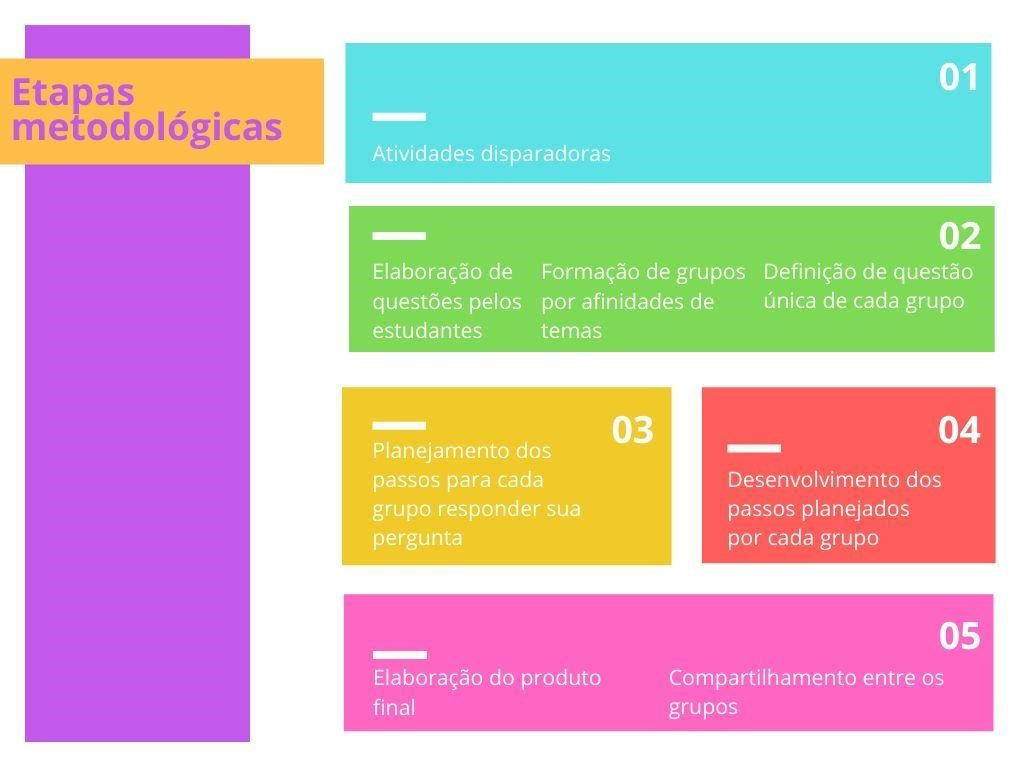
\includegraphics[width=400bp]{investigacao1.jpg}

\end{figure}

\begin{itemize}
\item \textbf{Atividades disparadoras}: Momento para conhecer materiais que lhe provequem um estranhamento (Para saber+: O cotidiano e seu estranhamento) daquilo que acontece em sua rotina e lhe permita iniciar questionamentos sobre ela. São materiais com otextos e/ou vídeos jornalísticos, materiais artísticos (como poesia, contos crônicas, apresentações, instalações, performances), depoimentos de seus colegas ou de outras pessoas da comunidade escolar, etc.

\item \textbf{Elaboração de questões e definições dos grupos de trabalho}: Momento para organizar as questões provenientes das atividades disparadoras em um problema geral que permita uma análise objetiva a partir do uso de indicadores. A formação de grupos pode lhes auxiliar a separar o problema geral em perguntas específicas e dividir tarefas com seus colegas.

\item \textbf{Planejamento da investigação}: A partir dos problemas colocados, você e seus colegas deverão se aprofundar nas ferramentas necessárias para a execução das pesquisa.

\item \textbf{Desenvolvimento da investigação}: Vocês efetivamente utilizarão os novos conhecimentos e provavelmente adquirão mais alguns. É nesta fase do trabalho que os conceitos apreendidos no momento anterior serão realmente aplicados, ganhando profundidade.

\item \textbf{Produto final}: Os grupos apresentarão a pesquisa de análise matemática em um formato concreto, compartilhando seus resultados com todos os colegas da comunidade escolar.
\end{itemize}

Ainda sobre os produtos conclusivos das pesquisas, o que se espera alcançar ao final é um estímula à pesquisa científica e ao exercício da intervenção prática sobre a realidade a partir de sua objetividade.

Esperamos que seja uma experiência rica de significado e possibilidade para você e todos os seus estudantes.

\know{O cotidiano e seu estranhamento}

De acordo com a filósofa húngara Agnes Heller, nossas vidas são marcadas profundamente pela dimensão do cotidiano. Como o próprio nome sugere, trata-se do momento da vida que nos ocupamos com nossa rotina diária. Quanto mais o tempo passa e, consequentemente, mantemos os elementos essenciais da rotina intocados, mais nos acostumamos a tratar tudo aquilo que nos acontece como algo "natural", como algo que não possuísse outra alternativa de ser.

<as a natureza, assim como a vida social, é bastante dinâmica. Basta prestarmos atenção ao nosso redor para identificarmos, tanto na natureza quanto na sociedade, formas bastante diferentes de manifestação da vida. Neste momento, podemos realizar um exercício de estranhamento, ou seja, de questionamento daquilo que está estabelecido e de proposição de algo diferente do corriqueiro.

\begin{knowledge}{O que isso, a conjuntura?}

O termo conjuntura se tornou recorrente na historiografia recente graças à figura de Fernand Braudel. Historiador franês vindulado à escola dos Annales, ele foi responsável por propor outro modelo de registro da história.

De uma disciplina atrelada aos estudos do passado, que buscava cada vez mais compreender o chamado tempo presente, Braudel vincula seu ofício a uma forma de compreensão mais ampla, agregando recursos de análise das ciências humanas em geral. 

De maneira bem resumida, para Braudel, seria possível realizar uma pesquisa historiográfica a partir de três níveis: estrutural, conjuntural e fatual. No primeiro seria possível observar fenômenos de longa duração, relações sociais e ambientais dos seres humanos que permanecem ativos por longos períodos. No conjuntural, são fenômenos de média duração, que não consolidam estruturas de relação, mas que não se resumem a meros acontecimentos pontuais, algo restrito ao entendimento da história fatual (aquela que se contenta, como o nome sugere, aos fatos, a imediaticidade das relações).

Portanto, quando nos referimos à conjuntura, estamos evocando a tentativa de avaliar um período histórico particular dentro de um estrutura estabelecida de relações.

\end{knowledge}

\explore{Primeiras informações sobre a pandemia}
\phantomsection\label{primeiras-informacoes}

Em dezembro de 2019, um novo coronavírus, chamado de Sars-Cov-2\footnote{Sars-Cov-2 é a abreviação, em inglês, para o coronavírus da síndrome respiratória aguda grave 2.}, causador da COVID-19\footnote{COVID-19 é a abreviação, em inglês, para a doença causada pelo novo coronavírus, iniciada em 2019}, foi identificado na cidade de Wuhan, na China. Desde então, o vírus tem se disseminado pelo mundo. O ritmo rápido do alastramento e o alto poder de contágio e de letalidade tem causado preocupações em todos. Em 11 de março de 2020, a Organização Mundial da Saúde (OMS) declarou que o mundo estava em uma pandemia, isto é, uma epidemia de proporções mundiais. Naquele momento, o relatório da OMS (Disponível em \url{https://www.who.int/emergencies/diseases/novel-coronavirus-2019/situation-reports/} apontava que o mundo tinha 118 319 casos confirmados e 4 292 mortes, sendo a maior parte na China, que tinha 80 955 casos confirmados e 3 162 mortes. Fora da China, a região mais afetada era a Itália, com 10 149 casos confirmados e 631 mortes. No Brasil tínhamos registrado oficialmente 35 casos e nenhuma morte (apesar de posteriormente o ministério da Saúde confirmar que o vírus já tinha causado mortes no país no mês de janeiro de 2020).

Apersar do vírus não escolher quem ele contamina, a dinâmica da propagação e as consequências da doença acometeu regiões do mundo de formas muito distintas. Fatores sociais, econômicos e culturais, bem como as táticas adotadas ao enfrentamento têm sido apontados como algumas das dimensões que impactam nessas diferênças.

Tudo isso parece distante para você? No caso de nosso país, será possível que a maneira como a COVID-19 se disseminou e foi tratada ocorreu de maneira similar em todo o território? E em sua cidade? Quais medidas de enfrentamento à doença você pode observar? Apresentaram eficiência? E como as pessoas mais próximas a você estão conseguindo sobreviver em condições de trabalho tão instáveis?

Vejamos algumas informações: No Brasil, até o dia 12 de maio de 2020, o ministério da saúde (\url{https://COVID.saude.gov.br/}) tinha registrado 177 589 casos, sendo 12 400 tinha falecido, 72 596 tinham se recuperado e 92 693 continuavam em acompanhamento.

Além dos números brutos, para dar uma dimensão da epidemia, auxiliar no acompanhamento da sua evolução e criar parâmetros para tomadas de decisão, o ministério da saúde calcula diversos indicadores. No Brasil\footnote{Segundo estimativa do IBGE, em 2019, o Brasil tinha 210 147 125 de habitantes.}, alguns dos indicadores, calculados com base nos dados do dia 12 de maio de 2020, são:

\begin{itemize}
\item \textbf{Coeficiente de Incidência}: É o número de casos de COVID-19 para cada 100 mil habitantes, em um determinado período de tempo. Calcula-se assim:

\begin{equation*}
\frac{\text{número de casos}}{\text{população}} \times \num{100000} = \frac{\num{177589}}{\num{210147125}} \times \num{100000} \approx 84,5
\end{equation*}

Esse número significa que, a cada 100 mil pessoas, 84,5 haviam sido acometidas pela COVID-19.

\item \textbf{Coeficiente de Mortalidade}: É o número de mortes para cada 100 mil habitantes, em um determinado período de tempo. Calcula-se assim:

\begin{equation*}
\frac{\text{número de óbitos}}{\text{população}} \times \num{100000} = \frac{\num{12.000}}{\num{210147125}}\times\num{100000}\approx 5,9
\end{equation*}

Esse número significa que, a cada 100 mil pessoas, 5,9 haviam morrido por causa da infecção pelo Sars-Cov-2.

\item \textbf{Taxa de Letalidade}: É o percentual, dentre todas as pessoas infectadas, que morreram por causa da doença. Calcula-se assim:

\begin{equation*}
\frac{\text{número de óbitos}}{\text{total de infectados}} = \frac{\num{12400}}{\num{177589}} \approx 0,698 = 6,98\%
\end{equation*}

Esse número significa que 6,98\% das pessoas infectadas até aquela data tinham morrido por causa da doença.

\end{itemize}

\know{As formas de enfrentamento à pandemia}

No primeiro epicentro da doença, a cidade de Wuha, por exemplo, antes mesmo de ser classificada como pandemia, a medida adotada foi a de uma rigorosa quarentena.

Na República da Coreia, uma tática foi a utilização do rastreamento da população através de GPS associada a uma campanha massiva de testes.

Em outros territórios, como o Vietnã, houve fechamento de fronteiras.

Para além do continente asiático, o mundo apresentou formas replicadas das estratégias acima mencionadas, mas com resultados bastante diferentes.


\begin{task}{Calculando e interpretando dados da COVID-19 por região}

A tabela a seguir apresenta o tamanho da população e os dados brutos do número de casos e de óbitos pela COVID-19 em cada região do Brasil no dia 12 de maio de 2020.

\begin{enumerate}
\item Complete a tabela calculando os coeficientes de indicência, de mortalidade e a taxa de letalidade de cada Estado.
\item Qual região era, até aquele momento, a mais afetada pela COVID-19? Justifique.
\item Você percebeu vantages e desvantagens de se utilizar os coeficientes e taxas? Quais?
\item Como a sua região estava afetada pela COVID-19 naquele momento? Faça a comparação com os dados de outras regiões.
\item Compartilhe suas descobertas com seus colegas.
\end{enumerate}

\begin{table}[H]
\centering
\setlength\tabcolsep{4pt}
\begin{tabu} to \textwidth{|c|r|r|r|r|r|r|}
\hline
\thead
Região & População & Casos & Óbitos & \makecell{Coeficiente de \\ Incidência} & \makecell{Coeficiente de \\ Mortalidade} & \makecell{Taxa de \\ Letalidade} \\
\hline
Centro-Oeste & 16 297 074 & 5 090 & 129 & & & \\
\hline
Nordeste & 57 072 654 & 58 316 & 3 568 & & & \\
\hline
Norte & 18 430 980 & 30 900 & 2 190 & & & \\
\hline
Sudeste & 88 371 433 & 74 727 & 6 216 & & & \\
\hline
Sul & 29 975 984 & 8 556 & 297 & & & \\
\hline
\end{tabu}
\caption{Fonte: \href{https://COVID.saude.gov.br/}{Ministério da Saúde} (Consulta em 12 de Maio de 2020)}
\end{table}
\end{task}

\explore{outras dimensões da epidemia}
	
Antes da pandemia chegar em terras tupiniquins, acompanhávamos os impactos catastróficos causados em outras regiões do mundo. Receosos, especulávamos sobre como, quando e em que medida ela atingiria nossa nação. Seria também catastrófica ou seria apenas uma gripezinha? Nosso sistema de saúde público conseguiria dar conta? Todos os indivíduos teriam o mesmo acesso ao tratamento? E os impactos em nossa economia? Quais setores produtivos seriam considerados essenciais para nossa sociedade? E aqueles setores produtivos seriam considerados essenciais para nossa sociedade? E aqueles trabalhadores de setores considerados essenciais para nossa sociedade? E aqueles trabalhadores de setores considerados não essenciais, como poderiam garantir o seu sustento? Sobre a estratégia do isolamento social, como colocá-la em prática em locais com grandes aglomerados de pessoas, como nas fabelas, nos presídios, etc? Resumindo, considerando a nossa estrutura socia, econômica e cultural, a pergunta geral era: como faríamos para enfrentar a pandemia?

Quando a doença deu seus primeiro sinais por aqui, essas questões começaram a ter respostas concretas. Pesquisadores de várias áreas, sobretudo nas universidades e insitutos de pesquisa trabalhavam arduamente para compreender o seu avanço.

O estudo da Funcação Oswaldo Cruz\footnote{Que pode ser acessado em \url{  https://agencia.fiocruz.br/estudo-aponta-maior-aceleracao-da-COVID-19-no-norte-e-nordeste}}, divulgado em 29 de maio, mostrou que o ritmo de aumento do avanço da COVID-19 nas regiões Norte e Nordeste foi muito maior do que no restante do país. O estudo sugeriu a existência de uma relação entre esse aumento e os recursos de cada região.

\begin{quote}
"O Amazonas passou de uma taxa de 493 casos por milhão de habitantes em abril, para 5 300 em maio. O Amapá passou de 492 para 5 100. Roraima, de 366 para 3 266 e Ceará, d3 356 para 3 078. Na comparação, estados com mais recursos parecem menos atingidos pela pandemia, como por exemplo o Paraná, onde a taxa passou de 86 para 217, e o Rio Grande do Sul, de 75 para 329."
\end{quote}

Ou \href{https://drive.google.com/file/d/1tSU7mV4OPnLRFMMY47JIXZgzkklvkydO/view }{estudo}, do Núcleo de Operações e Inteligência em Saúde (NOIS), da PUC-Rio, divulgado no dia 28 demaio, realizou uma análise socioeconômica da taxa de letalidade da COVID-19 no Brasil buscando mostrar que as altas taxas são influenciadas pelas desigualdades no acesso ao tratamento. Para chegas às conclusões, foram cruzadas informações obtidas em duas plataformas públicas: o \href{https://opendatasus.saude.gov.br/}{OpenDataSUS}, que traz dados sobre a saúde no Brasil, e o \href{http://atlasbrasil.org.br}{Atlas de Desenvolvimento Humando do Brasil}, que traz indicadores sociais e econômicos, como o Índice de Desenvolvimento Humano (IDH), o índice de Gini, o Índice de Vulnerabilidade Social, a distribuição da população por classe, gênero e raça, por nível de escolaridade entre outros.

Um dos gráficos apresentados por esse estudo, por exemplo, mostrou a proporção de óbitos ou recuperados por escolaridade e por Raça/Cor.

\begin{figure}[H]
\centering
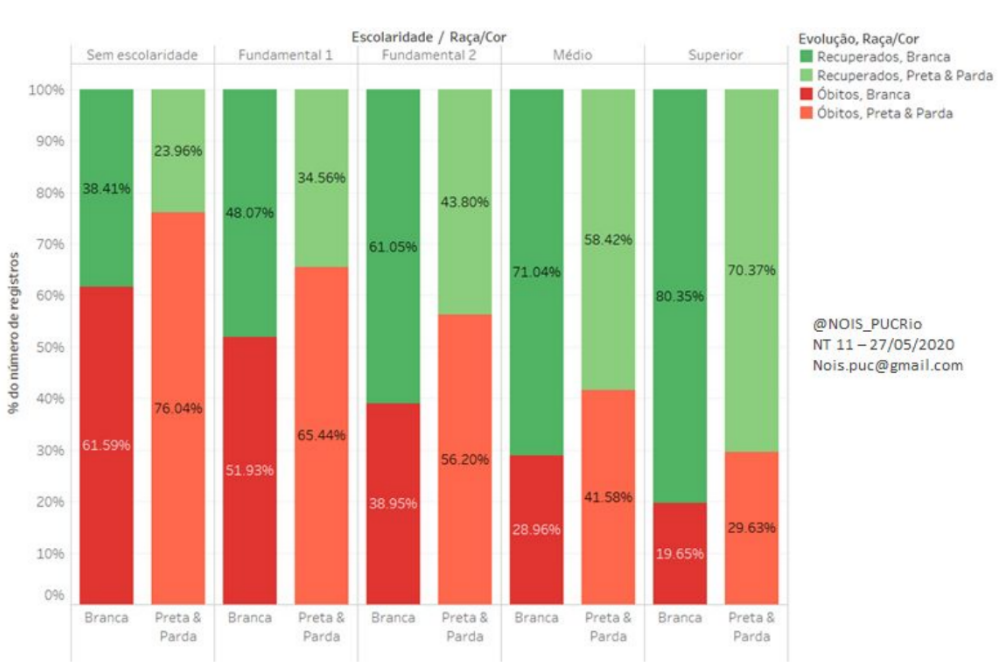
\includegraphics[width=400bp]{investigacao2}

\end{figure}

Impactos na economia também começaram a aparecer mais fortemente em indicadores como o Produto Interno Bruto (PIC) e as taxas de ocupação do trabalho. Em 29 de maio, o IBGE divulgou que "o PIB apresentou contração de 1,5\% na comparação do primeiro trimestre de 2020 contra o quarto trimestre de 2019, na série com ajuste sazonal. A Indústria (-1,4\%) e os Serviços (-1,6\%) apresentaram recuo, enquanto a Agropecuária (0,6\%) cresceu"\footnote{\url{https://agenciadenoticias.ibge.gov.br/agencia-sala-de-imprensa/2013-agencia-de-noticias/releases/27837-pib-cai-1-5-no-1-trimestre-de-2020}}. Quanto às taxas de ocupação do trabalho, dados da Pesquisa Nacional por Amostra de Domicílios Contínua (PNAD Contínua), revelaram que "a taxa de desocupação passou de 11,2\% para 12,6\% no trimstre terminado em abril, atingindo 12,8 milhões de desempregados"\footnote{\url{https://agenciadenoticias.ibge.gov.br/agencia-noticias/2012-agencia-de-noticias/noticias/27821-desemprego-atinge-12-6-no-trimestre-ate-abril-com-queda-recorde-na-ocupacao}}.

Como percebemos, os dados nos ajudam a compreender diversas dimensões de uma situação. Tratar de cada uma delas separadamente pode nos dar objetividade, mas certamente é insuficiente para propor soluções amplas. Por isso, podemos dividir tarefas para organizar essas informações, mas é sempre importante trocarmos experiências para compreender a situação de forma mais ampla e não cair em ilusões de soluções simplistas para problemas complexos.

\begin{task}{}

O texto acima trouxe a ideia de que podemos utilizar informações quantitativas e indicadores para compreender algumas dimensões dos problemas causados pela pandemia.

\begin{enumerate}
\item A seguir apresentamos as definições de alguns indicadores. Escreva como você imagina que cada um deles pode estar relacionado com a pandemia.

\begin{itemize}[itemsep=1em]
\setlength\parskip{-2pt}
\item \textbf{Pirâmide Etária}

\textbf{Descrição}: Quantidade de pessoas de uma região separadas por faixa etárias.

\textbf{Fonte}: IBGE - \href{https://www.ibge.gov.br/estatisticas/sociais/populacao/25089-censo-1991-6.html?=&t=o-que-e}{Censo} e \href{https://www.ibge.gov.br/estatisticas/sociais/populacao/9173-pesquisa-nacional-por-amostra-de-domicilios-continua-trimestral.html?t=destaques}{PNAD Contínua}

\item \textbf{Números de leitos hospitalares por habitante}

\textbf{Descrição}: Proporção do número de leitos hospitalares por habitante

\textbf{Fontes}: \href{https://datasus.saude.gov.br/}{Ministério da Saúde - DataSUS}; Secretarias de Saúde Estaduais e Municipais

\item \textbf{Índice de atendimento total de esgoto referido aos municípios atendidos com água}

\textbf{Descrição}: Percentual da população atendida por rede coletora de esgoto (com ou sem tratamento) em relação à população total.

\textbf{Fonte}:\href{http://www.snis.gov.br/painel-informacoes-saneamento-brasil/web/painel-setor-saneamento}{Sistema Nacional de Informações sobre Saneamento (SNIS)}

\item \textbf{Taxa de desocupação}

\textbf{Descrição}: Percentual de pessoas desocupadas em relação ao total de pessoas na força de trabalho.

\textbf{Fonte}: IBGE - \href{https://www.ibge.gov.br/estatisticas/sociais/populacao/9173-pesquisa-nacional-por-amostra-de-domicilios-continua-trimestral.html?t=destaques}{PNAD Contínua}

\item \textbf{Índice de Vulnerabilidade Social (IVS)}

\textbf{Descrição}: Indicador que sintetiza informações de infraestrutura, escolaridade e trabalho de grupos populacionais.

\textbf{Fonte}: \href{http://ivs.ipea.gov.br/index.php/pt/}{IPEA} (com dados do censo de IBGE)
\end{itemize}

\item Você conhece outras dimensões dos problemas causados pela pandemia? Que tipos de indicadores você acha que seriam importantes para analisar essas dimensões?

\end{enumerate}


\end{task}

\explore{O que é uma boa pergunta científica?}
\phantomsection\label{pergunta-cientifica}

Nós, seres humanos, podemos ser muito diferentes uns dos outros. No entanto, existe algo que nos unifica: absolutamente, todos nós temos problemas. Decerto, eles podem variar muito. Algumas pessoas precisam se preocupar constantemente com o trabalho que precisam executar para conseguir alguma remineração para comprar produtos jque consideram necessários a sua sobrevivência. Outras passam longe desse tipo de preocupação, mas muitas vezes não encontram sentido profundo em suas vidas, deprimindo-se.

Em ambos os casos, não há escapatória: se não podemos solucionar esses problemas seremos soterrados por eles. Portant, nosso cotidiano é uma dimensão da vida na qual precisamos constantemente dar respostas aos nosso problemas. De preferência, rapidamente, para que não se acumulem e nos prejudiquem.

Deste modo, a qualidade das nossas respostas interfere diretamente em nosso cotidiano. E conseguimos dar respostas melhores quando conseguimos entender melhor nossos problemas, quando conseguimos elaborá-los na forma de pergunts. Em outras palavras, conseguimos expressar nossa humanidade de maneira mais vívida quando somos curiosos.

Mas a velocidade exigida pelo cotidiano dificulta a formulação das perguntas. A necessidade de respostas rápidas desorienta nossos esforços em busca de exercitar nossa curiosidade. É por isso que outra dimensão da vida é imprescindível: a ciência.

Independentemente da área do conhecimento, o desenvolvimento científico é todo baseado em perguntas. Quando quere investigar algum processo, fenômeno ou aparato, os cientistas elabooram uma pergunta relacionada ao seu objeto/tema de estudo e se concentram nela. A dimensão científica privilegia o momento da pergunta e cuida para que haja tempo necessário para sua resposta. Diferentemente das pergundas cotidianas, as perguntas científicas precisam seguir certos critérios:

\begin{itemize}
\item elas devem ser quantitativas, ist é, devem estar relacionadas a quantidades e/ou informações numéricas;
\item precisam ser exequíveis num período de tempo apropriado (e por isso não podem demandar anárlises muito longas ou complexas);
\item é necessário que sejam comparativas, ou seja, avaliar diferentes situações ou a mesma situação em localidades diferentes, etc;
\item busquem ser interessantes, de forma que não sejam respondidas com uma simples busca na internet;
\item e sjeam simples, restritas a situações pouco complexas ou olhar para apenas um fator de uma determinada situação.
\end{itemize}

Vejamamos como podemos aplicar esses critérios em nosso exemplo. Abaixo temos uma tabela com exemplos de perguntas adequadas e inadequadas com relação a cada uma das características que você deve seguir:

\begin{table}[H]

\centering
\begin{tabu} to \textwidth{|c|>{\vspace{3pt}}m{.3\textwidth}<{\vspace{3pt}}|m{.3\textwidth}|}
\hline
\thead
Característica & Adequada & Inadequada \\
\hline
\cellcolor{white}\textcolor{black}{\textbf{Quantitativa}} & O índice de pessoas afetadas pela Covid em minha escola é maior ou menor do que na minha cidade? & Como se sentiram as pessoas infectadas em minha escola?\\
\hline
\cellcolor{white}\textcolor{black}{\textbf{\makecell{Exequível em \\ tempo apropriado}}} & Qual a taxa de ocupação das famílias de minha turma antes e depois da pandemia? & Qual a taxa de pessoas ocupadas em minha região antes e depois da pandemia? \\
\hline
\cellcolor{white}\textcolor{black}{\textbf{Comparativa}} & A taxa de letalidade da Covid é a mesma nas comunidades indígenas e nos grandes centros urbanos brasileiros? & A taxa de letalidade da Covid é a mesma para diferentes populações do Brasil?\\
\hline
\cellcolor{white}\textcolor{black}{\textbf{Sedutora/interessante}} & Qual foi o impacto da quarentena em minha região na contenção da pantemia? & Quam não tem acesso à rede de água e esgoto foi mais afetado pela Covid? \\
\hline
\cellcolor{white}\textcolor{black}{\textbf{Simples}} & Qual região da minha cidade apresentou a maior taxa de disseminação da Covid? & Qual a taxa de disseminação da Covid em minha turma? \\
\hline
\end{tabu}
\end{table}

Vejam que as perguntas da segunda coluna apresentam características que, embora não as tornem desnecessárias para a compreensão da realidade, as tornam inviáveis no contexto da sala de aula. Elas não permitem um aprofundamento metódico nos estudos matemáticos se estiverem orientadas a tentar compreender a subjetividade dos sujeitos envolvidos. Tampouco pode ser objetiva e, ao mesmo tempo, extremamtente abrangente, inviabilizando sua feitura nos prazos possíveis. O mesmo ponto sobre a abrangência vale para os casos de comparação possíveis: quanto mais genérica a comparação, mais difícil será efetivá-la. E, por fim, as perguntas não podem querer validar sua opinião, seja na confirmação de uma opinião amplamente aceita, seja na limitação rasteira do seu objeto.

Você não precisa se preocupar em tentar solucionar os grandes problemas do mundo. Pelo menos não por agora. Afinal, estas grandes questões demandam um esforço que foge aos limites da pesquisa em sala de aula.

Mas isso não significa que você deva abandonar esse desejo. Ao contrário, nossa intenção é que você seja cada vez mais capaz de alcançar essa possibilidade. Para isso, cabe um exercídio: dividir essa pergunta comiplexa em perguntas mais simples. Ao serem satisfatoriamente respondidas, nos enriquecem do conhecimento necessário para tratar de questões mais complexas, nos fazendo galgar degraus até nosso interesse final.

\begin{task}{Elaboração de boas perguntas científicas}

Elabore três perguntas investigadas sobre as pectos do seu tema. Tente seguir os critério mencionados anteriormente. Utilize as atividades dos Explorando "\hyperref[primeiras-informacoes]{Primeiras Informações Sobre a Pantemia}" e "Percebendo e medindo outras dimensões da pandemia" como inspiração. Naquelas atividades pudemos conferir como é possível alcançarmos os dados sobre a disseminação da pandemia por região, bem como avaliar os impacos de seu avanço a partir de índices que contemplam diversas dimensões da vida, como economia, saúde, educação, raça e gênero. Ao fazer as atividades e ler o texto daquela seção, quais curiosidades e questionamentos vêm à sua mente?

Uma dica: Ao pensar em perguntas tente imaginar como você faria para respondê-las. Que tipo de dados, medidas ou observações seria necessárias? Se você não souber por onde começar, provavelmente você pensou em uma pergunta é complexa.

Depois de verificar com sua professora ou seu professor se as três questões formuladas atendem todas as características para se enquadrarem como uma boa pergunta, é hora de definir qual será a sua pergunta de investigação.

Escreva em seu caderno a pergunta na qual você irá se aprofundar. Lembre-se que ela tem que atender a todas as características discutidas no texto "\hyperref[pergunta-cientifica]{O que é uma boa pergunta científica}".

\end{task}

\arrange{Planejando a investigação - hipóteses}

Depois de elaborada a pergutna, é hora de pensar em como respndê-la. Existe um ditado que expressa a seguinte ideia: só fazemos perguntas para as quais já temos condições de dar respostas. É provável que você, ao formular sua pergunta, já tenha um palpite do que pode ser a resposta. Ele pode parecer bastante coerente na sua mente, mas é possível que você não consiga expressá-lo em palavras com a mesma desenvoltura. Trata-se mais de intuição do que de raciocínio.

Considerando que a ciência é uma atividade que trabalha com explicações baseadas em evidências, é necessário testarmos nossas ideias intuitivas por meio de observações ou tomadas e análises de dados. Um projeto científico possui esta finalidade: confrontar o pensamento intuitivo com a reaidade, demonstrando o alcance de uma certa resposta ao problema colocado a partir de um conjunto de etapas passíveis de serem reproduzidas (verificadas) por outras pessoas.

A primeira etapa de uma investigação é entender o que você imagina como respota para sua pergutna, ou seja, materializar uma intuição em linguagem conteitual, formular aquilo que chamamos de hipótese. Por exemplo, para a pergunta "\textit{A taxa de letalidade da COVID-19 é a mesma nas comunidades indígenas e nos grandes centros urbanos brasileiros}"{}, uma hipótese possível é que sim, pois somos todos seres vivos da mesm espécie. Mas uma outra hipótese possível é de que diferentes populações são suscetíveis a doenças diferentes, pois entraram em contato com vírus e bactérias diferentes ao longo de sua formação histórica.

\begin{task}{Planejando a investigação}

Agora é sua vez!

Escreva as hipóteses que vocêm tem sobre a pergunta que escolhei investigar.

\end{task}

\arrange{uso de indicadores}

As explicações que construímos sobre a realidade passa, necessariamente, pelas ações de identificar e comparar. Percebemos a existência de diferenças e, em seguida, buscamos um jeito de compará-las, usando essas informações para então construir nossas explicações. Uma forma de fazer isso é através da utilização de indicadores.

Um indicador é, a grosso modo, um recurso metodológico. Para nossos propósitos, nos interessa que ele seja empiricamente aferido, quantitativo, e que sintetize informações sobre aspectos da realidade ou sobre suas transformações. Um indicador com essas características procura dar objetividade a um conceito que pode ser, a princípio, abstrato.

Podemos representar sua construção em basicamente três etapas:

\begin{enumerate}[label=\arabic* -]
\item percepção de eventos empíricos da realidade;
\item obtenção de dados brutos e estatísticas sobre o evento;
\item sintetização dos dados procurando dar-lhes um valor informacional sobre certos contextos.
\end{enumerate}

\begin{figure}[H]
\centering

\begin{tikzpicture}[every node/.style={scale=.9}]
\tikzstyle{quad}=[draw, rectangle, node distance=6cm, align=center, minimum height=2.5cm, minimum width=4cm];

\node (a) [quad] {Eventos \\ empíricos \\ da realidade};
\node (b) [quad, right of=a] {Obtenção \\ de dados \\ brutos e \\ estatísticas};
\node (c) [quad, right of=b] {Sintetização e \\ agregação de valor \\ informacional para \\ analisar contextos};

\path[->,very thick]
(a) edge (b)
(b) edge (c);
\end{tikzpicture}

\end{figure}

Apesar da busca de objetividade, não podemos esquecer que a construção de qualquer indicador é realizada por grupos de indivíduos influenciados histórica e socialmente, e que portanto colocam nesses indicadoeres determinadas visões de mundo. Desta forma, um indicaodr pode ser objetivo, mas jamais é neutro ou imparcial.

Vejamos a seguir alguns exemplos de indicadores e seus processos de construção, incluindo desde influências que moldam as percepções da realidade, até os processos técnicos de cálculo.

\begin{example}{Taxas de subutilização na força de trabalho}

A elaboração dessa taxa parte da percepção de que existem pessoas desempregadas e que querem trabalhar, e também de pessoas que poderiam trabalhar mais do que estão efetivamente trabalhando. Essa taxa pode indicar quanta força de trabalho é desperdiçada. Para buscar dados concretos sobre essa ideia, primeiro é preciso definir quais pessoas integram a força de trabalho e quando são consideredas subutilizadas. O IBGE define esses termos da seguinte forma:

\begin{itemize}
\item \textbf{Força de trabalho}: Pessoas com mais de 14 anos de idade que estão dispostas a trabalhar.
\item \textbf{População Subutilizada}: São pessoas que estão dispostas a trabalhar mas não conseguem emprego ou trabalham menos do que poderiam. São separadas em quatro grupos:
	\begin{itemize}
	\item \textbf{Desocupadas}: Pessoas que não têm trabalho nenhum e que estão efetivamente em busca de conseguir um trabalho.
	\item \textbf{Subocupadas}: Pessoas que trabalham menos de 40 horas na semana, mas que estão dispostas a trabalhar mais.\
	\item \textbf{Deslentadas}: Pessoas desempregadas, que gostariam de trabalhar, mas que perderam as esperanças de conseguir um trabalho.
	\item \textbf{Não podem assumir}: Pessoas que gostariam de trabalhar, mas que não podem assumir um emprego por algum motivo
	\end{itemize}
\end{itemize}

A tabela a seguir mostra os dados da \href{ftp://ftp.ibge.gov.br/Trabalho_e_Rendimento/Pesquisa_Nacional_por_Amostra_de_Domicilios_continua/Mensal/Quadro_Sintetico/2020/pnadc_202004_quadroSintetico.pdf}{PNAD contínua do trimestre fevereio/março/abril de 2020} referente a esses grupos:

\begin{table}[H]
\centering
\begin{tabu} to \textwidth{|l|c|c|}
\hline
\thead
Grupo & \makecell{Total \\ (em milhões de pessoas)} & \makecell{Taxas \\ (em \% da Força de Trabalho)} \\
\hline
Força de Trabalho & 102,1 & 100\% \\
\hline
Desocupados & 12,9 & 12,6\% \\
\hline
Subocupados & 6,1 & 6,0\% \\
\hline
Desalentados & 5,0 & 4,9\% \\
\hline
Não podem assumir & 4,7 & 4,6\% \\
\hline
População Subutilizada & 28,7 & 28,1\% \\
\hline
\end{tabu}
\end{table}

\end{example}

\begin{task}{Calculando e comparando indicadores}

A tabela a seguir apresenta os dados de subutilização da força de trabalho dos trimestres fev-mar-abr/2019 e nov-dez-jan/2020.

\begin{table}[H]
\centering
\begin{tabu} to \textwidth{|l|c|c|c|}
\hline
\thead
Grupo & \makecell{Fev-Mar-Abr/2019 \\ (em milhões \\ de pessoas)} & \makecell{Nov-Dez-Jan/2019 \\ (em milhões \\ de pessoas)} & \makecell{Fev-Mar-Abr/2020 \\ (em milhões \\ de pessoas)} \\
\hline
Força de Trabalho & 105,5 & 106,1 & 102,1 \\
\hline
Desocupados & 13,2 & 11,9 & 12,9 \\
\hline
Subocupados & 7,0 & 6,6 & 6,1 \\
\hline
Desalentados & 4,9 & 4,7 & 5,0 \\
\hline
Não podem assumir & 3,3 & 3,2 & 4,7 \\
\hline
População Subutilizada & 28,4 & 26,4 & 28,7 \\
\hline
\end{tabu}
\end{table}

\end{task}

\begin{enumerate}
\item Quais eram as taxas de subutilização na força de trabalho nos trimestres Fev-Mar-Abr/2019, Nov-Dez-Jan/2019 e Fev-Mar-Abr/2020?

\item O IBGE considera como força de trabalho potencial o grupo dos desalentados junto com aqueles que não podem assumir. O que você pode dizer sobre as variações da força de trabalho potencial nos trimestres apresentados?
\end{enumerate}

\arrange{apresentação de dados}

As tabelas e os gráficos são formas visuais de organizar informações quantitativas. Estes instrumentos são muito úteis para resumir informações e apresentá-las para uma leitura rápida. Entretanto, cada um desses instrumentos têm usos diferentes.

Por exemplo, as \textbf{tabelas} têm como principal função resumir uma grande quantidade de dados, de forma organizada.

Observe a imagem abaixo, de uma tabela do portal de dados \url{Brasil.io}. Ela apresenta oito tipos diferentes de informações, cada um para nove cidades brasileiras. Ou seja, esta tabela apresenta de forma compacta 72 dados.

\begin{table}[H]
\centering
\setlength\tabcolsep{2.5pt}
\setlength\tabulinesep{3pt}
\begin{tabu} to \textwidth{|l|l|c|r|r|r|r|r|}
\hline
\multicolumn{8}{|c|}{\cellcolor{\currentcolor!80}\textcolor{white}{\textbf{COVID-19 - Dados por Município}}} \\
\hline
\thead
Data & Município & UF & Confirmados & \makecell{Confirmados\\por 100k hab.} & Óbitos & Letalidade & \makecell{Óbitos por\\ 100k hab.}\\
\hline
30/05/2020 & São Paulo & SP & 58 619 & 478,44 & 4 239 & 7,23\% & 34,60 \\
\hline
29/05/2020 & Rio de Janeiro & RJ & 27 311 & 406, 28 & 3 430 & 12,56\% & 51,05 \\
\hline
30/05/2020 & Fortaleza & CE & 23 378 & 875,80 & 1 939 & 8,29\% & 72,64 \\
\hline
29/05/2020 & Manaus & AM & 17 492 & 801,37 & 1 349 & 7,71\% & 61,80 \\
\hline
30/05/2020 & Recife & PE & 14 832 & 901,24 & 1 040 & 7,01\% & 63,19 \\
\hline
29/05/2020 & Belém & PA & 11 509 & 771,00 & 1 311 & 11,39\% & 87,82 \\
\hline
29/05/2020 & Salvador & BA & 10 353 & 360,44 & 421 & 4,07\% & 14,66 \\
\hline
29/05/2020 & São Luís & MA & 8 882 & 806,07 & 521 & 5,87\% & 47,28 \\
\hline
29/05/2020 & Brasília & DF & 7 877 & 261,24 & 142 & 1,80\% & 4,71 \\
\hline
\end{tabu}

\caption*{Adaptado de \url{https://brasil.io/covid19/} - Acesso em 31/05/2020}
\end{table}

Um outro exemplo são os dados de disponibilidade de leitos de UTI e leitos clínicos apresentados nos boletins diários publicados pelo estado do Maranhão durante os primeiros meses de pandemia do novo coronavírus no Brasil.

Neste caso, a tabela tem a função de rapidamente passar informações importantes, como a taxa de ocupação de leitos na Grande Ilha, que inclui as cidades de São Luís e São José de Ribamar.

\begin{table}[H]
\centering
\begin{tabu} to \textwidth{|c|r|c|r|}
\hline
\multicolumn{4}{|c|}{\cellcolor{\currentcolor!80}{\textcolor{white}{\textbf{Leitos - Grande Ilha}}}} \\
\hline
\multicolumn{2}{|c}{\cellcolor{\currentcolor!80}{\textcolor{white}{\textbf{\makecell{Taxa de Ocupação de Leitos de UTI \\ Exclusivos Covid-19*}}}}} & \multicolumn{2}{|c|}{\cellcolor{\currentcolor!80}{\textcolor{white}{\textbf{\makecell{Taxa de Ocupação de Leitos de Clínicos \\ Exclusivos Covid-19*}}}}} \\
\hline
Total de Leitos & 240 & Total de Leitos & 752 \\
\hline
Leitos Ocupados & 230 & Leitos Ocupados & 304 \\
\hline
Leitos Livres & 10 & Leitos Ocupados & 448 \\
\hline
Taxa de ocupação & 95,83\% & Taxa de Ocupação & 40,43\% \\
\hline
\end{tabu}
\caption*{
\footnotesize
*Taxa de ocupação relativa aos leitos SUS disponíveis na rede SES/ME

Dados publicados pela Secretaria Estadual de Saúde do Maranhão

Boletim epidemiológico de 30/05/2020}
\end{table}

Os \textbf{gráficos de linha} são utilizados para mostrar evolução. Ele é o instrumento mais adequaod para, por exemplo, mostrar a evolução do total de casos de COVID-19 no Brasil em função do empo, como no gráfico da imagem a seguir, publicado pelo Ministério da Saúde em 31/05/2020.

\begin{figure}[H]
\centering
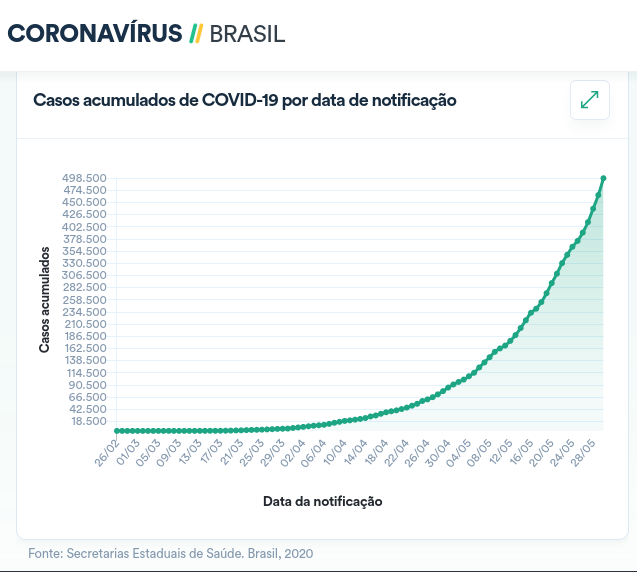
\includegraphics[width=400bp]{investigacao3}

\end{figure}

Ou ainda, para mostrar como evoluiu o índice de isolamento no Estado de São Paulo entre os meses de março e maio de 2020.

\begin{figure}[H]
\centering
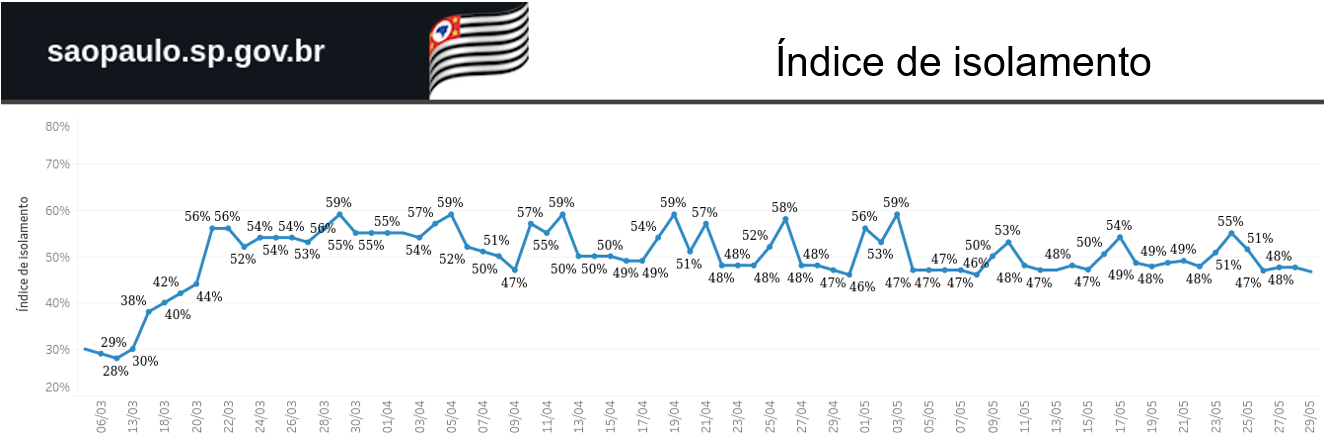
\includegraphics[width=400bp]{investigacao4}

\caption*{Fonte: Secretaria de Saúde do Estado de São Paulo. Acesso em 31/05/2020}
\end{figure}

Já os \textbf{gráficos de barras e colunas} são mais adequados para mostrar comparação entre quantidades. Um bom exemplo é o gráfico apresentado pelo Portal de Transparência de Registro Civil, que apresenta uma comparação da quantidade de óbitos com suspeita ou confirmação de COVID-19 por sexo e faixa etária.

\begin{figure}[H]
\centering
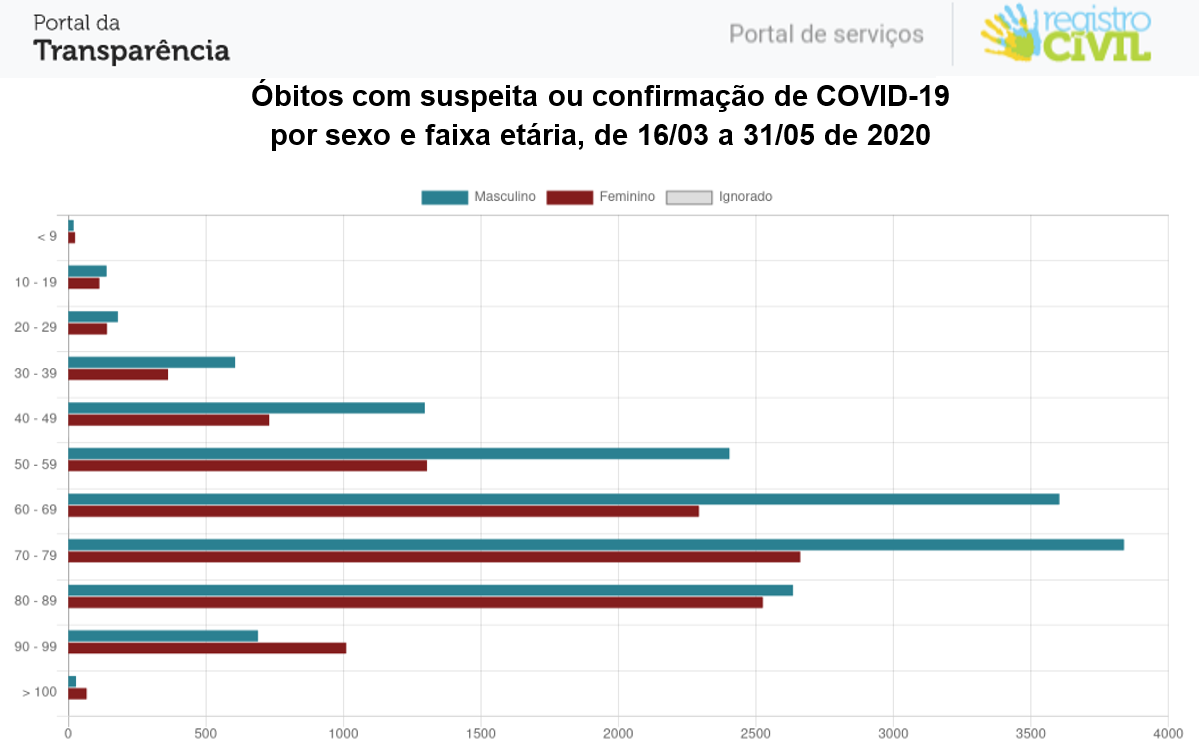
\includegraphics[width=400bp]{investigacao5}

\caption{Fonte: Central de Informações do Registro Civil - CRC Nacional}
\end{figure}

Os \textbf{gráficos de setores} dão noção de parte e todo, e por isso muitas vezes seus valores são apresentados na forma percentual. Esta foi a forma como o Estado de Santa Catarina escolheu para mostrar em seus boletins epidemiológicos a taxa de ocupação dos leitos de UTI. Repare como com este tipo de gráfico fica fácil entender se, comparado com o total de leitos, há muitos ou poucos livres.

\begin{figure}[H]
\centering
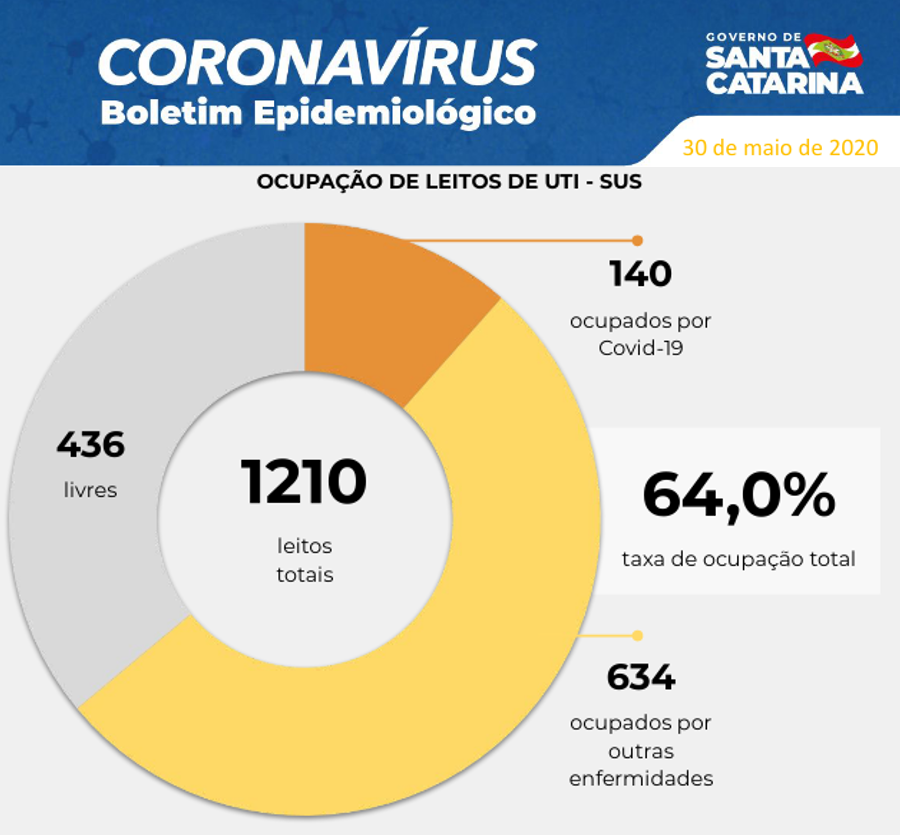
\includegraphics[width=300bp]{investigacao6}

\end{figure}


Existem muitas outras formas de mostrar dados quantitativos de formas visuais. Com os programas de edição de imagem, hoje em dia até existe um profissional que é especializado em elaborar gráficos, tabelas e diagramas que ajudem os leitores a entenderem melhor as informações de uma certa notícia ou relatório. Para elaborar um bom gráfico é necessário conhecimento matemático, compreensão de qual informação quer-se enfatizar e muita criatividade!

\arrange{fontes confiáveis}

A pesquisa científica se diferencia do nosso conhecimento cotidiano pelo método e pela busca apurada de fontes de informação. Não há atividade de pesquisa sem coleta de dados, sejam quantitativos ou qualitativos. Estes ainda podem ser divididos em três grupos:

\begin{itemize}
\item \textbf{Fontes primárias}: também chamadas de originais, são objetos relacionados à temática da pesquisa que não apresentam nenhuma leitura anterior. Pode se tratar de um documento (como um manuscrito ou texto de lei), imagem (fotografia), ou qualquer outra fonte de informação resultado de trabalho próprio ou de outrem reconhecido pela comunidade científica (como diários de pesquisa).
\item \textbf{Fontes secundárias}: busca apresentar uma análise sobre um material até então original. Ou seja, quem as utiliza alcança seu objeto de pesquisa a partir da avaliação de outra pessoa (como livros ou artigos científicos), mesmo que esta possa ter se equivocado na coleta dos dados ou na análise das informações.
\item \textbf{Fontes terciárias}: podem ser consideradas a combinação das duas formas anteriores. Compilados que buscam confrontar as fontes primárias com as secundárias, facilitando a pesquisa de interessados (como nas coletâneas). No entanto, estes terão de lidar com os limites do trabalho do responsável pela compilação.
\end{itemize}

A utilização desse tipo de fonte variará de acordo com as possibilidades de coleta de informações por parte do sujeito pesquisador. Você já deve ter percebido pelas descrições acima que as fontes primárias devem ser sempre preferidas. Muito embora sejam difíceis de ser apuradas, dependendo do local de onde se realiza a pesquisa, do seu momento histórico e do acesso à tecnologia necessária para sua interpretação, elas possibilitam um contato mais fiel ao objeto investigado.

A necessidade de fidelidade ao objeto está diretamente conectada ao fazer científico. Dados inconsistentes com a realidade afastam o pesquisador de seu objetivo, a lembrar, botar a prova um hipótese calcada, a princípio, no senso-comum cotidiano. Gastar tempo e energia para realizar uma atividade metódica que chegará a um resultado que poderia ser obtido por meio de raciocínios rápidos de nossa rotina é um desperdício que não pode ser permitido.

Portanto, faz parte da pesquisa apurar o grau de confiabilidade de suas fontes. Caso você e sua equipe não sejam capazes de realizar o próprio processo de coleta de dados, existem outras fontes de dados oficiais que podem atender às suas expectativas.

A dica é sempre procurar instituições de pesquisa reconhecidas. Estas costumam estar vinculadas às universidades públicas (no caso brasileiro) e ao Estado, nas esferas vinculadas às universidades públicas (no caso brasileiro) e ao Estado, nas esferas municipal, estadual e federal. Sobre o tratamento de dados socioeconômicos, temos o \href{https://www.ibge.gov.br/}{IBGE}. Já para dados relacionados à pandemia, o Ministério da Saúde elaborou um \href{https://covid.saude.gov.br/}{Painel Coronavírus}. Sua confiabilidade está ligada à dedicação exclusiva de seus trabalhadores nas atividades de pesquisa científica no seu histórico de análises ao longo dos anos e na importância que os dados produzidos por ele possuem para o encaminhamento consequente das políticas públicas estatais.

Se não for possível averiguar a confiabilidade da fonte, é possível proceder a pesquisa, desde que na elaboração de seu produto final isto seja publicizado. Ser honesto sobre a característica das fontes utilizadas, bem como sobre o procedimento de análise delas, permitirá a comunidade escolar e científica que se interesse por sua pesquisa colocar a prova seus resultados replicando o seu procedimento.

\know{Senso-comum e "fake news"}

Como vimos anteriormente, o conhecimento científico é important para colocar à prova nossas avaliações mais imediatas sobre a realidade. Podemos reconhecer que este conhecimento cotidiano, popularmente conhecido como senso-comum, ao ser exercitado em contraponto ao conhecimento científico, pode se tornar mais amparado neste último.

Não é exatamente o que se verifica desde há muito tempo. Poucas vezes o senso comum esteve alinhado com a ciência. Atividade realizada por grupos sociais específicos, geralmente as classes dominantes de uma determinada formação social, a ciência só se tornou mais próxima do cotidiano da maior parte da população com o espalhamento e a predominância da atividade industrial a nível mundial. E não necessariamente na atividade de pesquisa, mas no consumo de produtos desenvolvidos a partir de experiências laboratoriais.

Este afastamenteo entre ciência e senso-comum permitiu a fertilização do terreno de posturas e opiniões sobre a realidade baseadas em superstição e demagogia. Atualmente a disseminação de ideias que não encontram respaldo nas pesquisas científicas ou na verificação apurada dos fatos leva o nome genérico de \textit{fake news}.

É bem verdade que o fenômeno das \textit{fake news} envolve relações que estão além da relação entre ciência e senso-comum. Existe certo consenso sobre o quanto a atividade de disseminação de informações falsas serve a interesses políticos e também à manutenção de atividades econômicas diversas, a despeito do seu impacto negativo.

\know{adulteração de resultados e plágio}

Todo começo é difícil, em qualquer ciência. A necessidade de cumprir prazos e apresentar resultados parece dificultar ainda mais. Nada que a constante prática não seja capaz de superar. No entanto, muitas vezes, dadas as exigências de prestação de contas e de uma cultura de supervalorização do sucesso, pesquisadores se sintam tentados a adulterar os resultados para atender determinados interesses. Seja os daqueles que financiam suas atividades, seja os seus próprios, tentando fazer valer sua hipótese a despeito daquilo que a própria realidade apresenta, seja pela desqualificação em sua formação.

Outro fenômeno comum aos descaminhos da atividade científica, muito comum nas escolas, é o do plágio. Embora copiar, em parte ou totalmente, o texto produzido por outra pessoa não seja novo, a circulação de informações propiciada pelo advento da internet, associada às pressões comuns aos estudantes, o fez aumentar consideravelmente.

\begin{reflection}{A objetividade do conhecimento científico}

O avanço do fenômeno das \textit{fake news} e a existência das adulterações e plágios na pesquisa científica parece homogeneizar as maneiras como nós temos de produzir conhecimento. Tudo parece permitido e, em certa medida, válido para compreender a realidade. Será mesmo?

O termo objetividade é utilizado para apontar aquilo que um objeto de estudo é, independente da vontade ou do desejo da pessoa sujeito da pesquisa. Muitas vezes, quando falamos em objetividade na ciência, estamos falando no exercício de afastarmos nossos pré-julgamentos da atividade da pesquisa, tentando garantir melhores condições para botarmos à prova nossas hipóteses.

Mas, desde o início de nossas atividades nesta seção, priorizamos o exercício de estranharmos nossa realidade, partindo daquilo que há de mais pessoal em nossa rotina. Como podemos ser objetivos considerando todos os valores e conhecimentos do senso-comum vindos de nosso cotidiano?

É importante revermos a noção de objetividade como sinônimo de afastamento de nossos pressupostos. Como apontamos desde o início, a atividade da pesquisa precisa, para comuprir sua função de atividade metódica, confrontar o senso-comum, e não afastá-lo. Resumindo em uma palavra, ela precisa ser crítica.

Em todo o momento da pesquisa, desde a investigação até a sua apresentação , é important informar quais foram os caminhos tratados, quais os interesses que justificam essa pesquisa e como o resultado final corresponde ou não a à hipótese apresentada.

Á objetividade do conhecimento científico, tratado como um exercício amparado de avaliação coletiva, deveria primar não pela ideia da afastamento dos valores do pesquisador, mas pela exposição mais honesta possível de seus fundamentos.

\end{reflection}

\begin{task}{planejando a investigação}

A seguir você encontrará algumas perguntas orientadores para a formulação do planejamento. Em conjunto com seu grupo você deve responder cada uma das questões, registrando suas respostas em uma ficha ou no caderno.

\begin{enumerate}
\item A partir de notícias e outras fontes de informação sobre o tema de sua pergunta faça uma pesquisa e registre quais são os principais indicadores deste tema.
\item Quais dados você usará para responder a questão proposta? Justifique explicando a relação entre os dados exolhidos por você e a relação dele com a sua pergunta.
\item Quais as fontes de dados confiáveis para os dados escolhidos por você?
\item Explique como você utilizará os dados para responder a sua pergunta. Dê exemplos. Que cálculos você fará com esses dados e o que espera obter? Não se esqueça que ao final, sua análise deve servir para testar a sua hipótese inicial.
\item Faça um esboço do(s) tipo(s) de gráfico(s) que você utilizará para apresentar seus dados. Abuse das cores e criatividade em seu esboço. Não se esqueça de identificar quais dados você espera apresentar em cada gráfico que fizer.
\end{enumerate}

\end{task}

\practice{Mão na massa!}

Agora é hora de colocar em prática o seu planejamento!

Mas antes de iniciar o trabalho pense sobre como organizá-lo. Onde os dados dos índices ficarão guardados? Onde você fará suas contas e seus gráficos? Vai utilizar um caderno ou uma planilha? Onde anotará novas fontes bibliográficas que for encontrado pelo caminho, seus resultados parciais e conclusões? Em trabalhos em grupos é necessário também pensar em estratégias para que todos tenham acesso a todos os dados, contas, resultados e conclusões.

Uma boa estratégia é manter um diário de bordo no qua, ao final de cada aula, você escreve um pequeno parágrafo contando o que fez nela, os avanços e os próximos passos. Este diário pode ser feito num caderno próprio ou ser um relato coletivo.

As questões a seguir são uma síntese do que deve ser o seu resultado final. Você só conseguirá respondê-las em seu caderno quando finalizar sua pesquisa.

Mão à obra!

\begin{enumerate}
\item Como os indicadores, gráficos e tabelas que você construiu responndem a sua pergunta de investigação?
\item Você considera que os indicadores que você escolheu usar foram realmente adequados? Eles te ajudaram a responder sua pergunta? Justifique sua resposta.
\item Por último, escreva suas conclusões. É o resumo do que você aprendeu e do que se pode saber através desta investigação. Pode ser apenas uma frase e algumas vezes pode haver mais de uma concluão. É muito importante que na conclusão você analise a sua hipótese inicial. Ela estava correta? Se não estava, o que os dados mostraram de diferente das suas expectativas iniciais?
\end{enumerate}

\explore{o produto final}

Agora é  hora de materializar todo o seu aprendizado em um produto final. As possibilidades são ilimitadas e dependem da criatividade e de recursos (como tempo para execução, acesso a computadores e internet, disponibilidade de material, papel, tinta e etc.).

Algumas possibilidades são:

\begin{itemize}
\item um revista "científica" com os artigos dos grupos;
\item um congresso com um seminário de cada "grupo de pesquisa";
\item uma série de podcasts no qual cada grupo faz o seu programa;
\item um telejornal ou um canal com vídeos de cada grupo;
\item uma página de internet para cada grupo apresentar suas descobertas sobre o tema estudado;
\item um fazine ou uma HQ;
\item um panfleto ou um folder;
\end{itemize}

\begin{task}{refletindo sobre o produto final}

Vamos pensar um pouco sobre o que é important que haja nesse produto final. Realize em uma ficha ou em seu caderno os registros para as questões a seguir.

\begin{itemize}
\item Pesquise e discuta com colegas quais as principais características do tipo de produto final escolhido para ser realizado como finalização deste projeto de investigação. Registre em uma ficha ou em seu caderno os pontos de atenção para produzir um bom produto final.
\item Quem é o público alvo de seu produto final?
\item Quais são as informações mais importantes de sua investigação. Isto é, o que seu público alvo precisa aprender com seu produto final?
\end{itemize}

Agora é hora de efetivamente dar vida ao produto final. Após ele ficar pronto e ser compartilhado com seus colegas. Volte para responder às últimas pergutnas desta Unidade Temática.

\begin{itemize}
\item Como foi ver o seu produto final concretizado? O que você sentiu? O que acha que ficou bom e o que poderia ser melhorado?
\item O que você sente que aprendeu durante todo esse processo de investigação?
\item O que você achou de toda essa experiência?
\end{itemize}

\end{task}